\documentclass{article}

\usepackage[final]{neurips_2025}

\usepackage[utf8]{inputenc}
\usepackage[T1]{fontenc}
\usepackage{hyperref}
\usepackage{url}
\usepackage{booktabs}
\usepackage{amsfonts}
\usepackage{amsmath}
\usepackage{nicefrac}
\usepackage{microtype}
\usepackage{xcolor}
\usepackage{graphicx}
\usepackage{multirow}
\usepackage{array}
\usepackage{caption}
\usepackage{subcaption}

\title{Routing Cross-Region {LLM} Serving on Production Traces:\\Joint Cache, Network, and Queue Optimization Beats Per-Signal Heuristics}

\author{%
  Anonymous Author(s)\\
  Affiliation\\
  Address\\
  \texttt{email}\\
}

\begin{document}

\maketitle

\begin{abstract}
In cross-region LLM serving, time-to-first-token (TTFT) is highly sensitive to per-request routing decisions. KV-cache reuse across replicas can eliminate much of the prefill computation on multi-turn workloads, but realizing this potential requires jointly balancing cache locality against replica load and network cost. Additionally, public datasets to evaluate these policies do not represent long-context, high prefix-reuse workloads: LMSYS and WildChat average 2 and 2.5 turns per conversation, 0.5 and 2.9k tokens per request, and 5\% and 9\% intra-user reuse, respectively. To capture the setting where a majority of requests contain reusable prefixes, we evaluate common routing policies such as least-load, prefix-aware, session-affinity, and others on traces from a production inference endpoint featuring multi-turn conversations ($\sim$82 requests/user), $7$--$45\times$ longer prompts (21k average tokens), and $2$--$6\times$ higher KV-cache reuse (55\%). We evaluate policies on a multi-region GPU cluster where cross-region network latency ranges from 26\,ms to 466\,ms across replicas to test GORGO, a policy family that jointly optimizes cache reuse, network latency, and queue depth with weights tuned online to minimize p95 TTFT with no offline profiling. GORGO achieves the lowest TTFT at every percentile (p50, p95, p99) across both a tuning window and a held-out evaluation window against all other load-balancing policies, highlighting the impact of online joint optimization.
\end{abstract}

\section{Introduction}
\label{sec:intro}

Modern LLM chat services serve interactive workloads where the perceived latency is dominated by time-to-first-token (TTFT). On a single replica, TTFT is the sum of three contributions: (i) the network round-trip from the client (or proxy) to the replica, (ii) any time the request waits behind in-flight or queued requests, and (iii) the prefill computation needed to fill the KV cache for the input prompt. Modern inference engines such as SGLang and vLLM \citep{sglang2024,vllm2023} expose RadixAttention-style prefix caches that let an incoming request skip the prefill for any token prefix already cached on the replica that handles it. When prompts are long and prefixes are widely reused, this saving dominates: a 20{,}000-token prompt that hits a 90\% prefix match has only $\sim$2{,}000 tokens to prefill. The remaining computation can be served at decode-stage latencies even if the original prefill took seconds.

The KV-cache reuse opportunity, however, is contingent on routing. If a request is sent to a replica that has not seen its prefix, the saving is forfeit. If many requests are routed to the same warm replica, that replica becomes a queueing bottleneck and the cache hit no longer pays for itself. If the closest replica with a warm cache is on the other side of the world, the network round-trip can swallow what the cache hit was supposed to save. The routing layer of an LLM gateway therefore has to balance three terms simultaneously: the network distance to the replica, the load already on it, and the reusable cache state it holds for the incoming prompt. Each of the three is straightforward to optimize in isolation; the difficulty is the joint optimum, which depends on per-replica hardware, the prompt distribution, and the time-varying load.

The standard heuristics --- least-request, least-load, prefix-aware routing, session-affinity --- each pick exactly one of these signals and ignore the others. For workloads with weak prefix reuse and uniform replica latencies these heuristics work well \citep{nginx2024}. The interactive long-context regime breaks both assumptions. Production chat traffic to a long-context model concentrates most tokens in a small set of returning users with substantial prefix overlap, and replicas placed in different regions to follow user demand have round-trip times that differ by an order of magnitude. The right routing target for a given request can change from one minute to the next as load shifts, and weighting these three terms with a static rule of thumb leaves performance on the table.

Two further factors make this harder to evaluate empirically. First, the public chat datasets that have anchored most prior LLM-serving evaluations underrepresent long-context multi-turn traffic with reusable prefixes. We characterize this gap quantitatively below: LMSYS-Chat-1M and WildChat-4.8M average 470 and 2{,}900 tokens per request, with intra-user prefix reuse below 10\%. A production inference endpoint we replay carries 21{,}000 tokens per request on average and 53.7\% intra-user prefix reuse measured by a token-weighted prefix trie. Policies optimized for or evaluated only on the public sets do not see the regime where joint cache--network--queue trade-offs dominate TTFT. Second, the evaluation methodology itself matters: a routing policy that wins p50 by herding traffic onto a single warm replica typically loses on tail latency once that replica saturates. Reporting only one percentile hides this trade-off.

Our contributions are:

\begin{itemize}
\item A workload characterization (\S\ref{sec:characterization}) that places three datasets --- LMSYS-Chat-1M, WildChat-4.8M, and a 411{,}000-request, 4{,}984-user production trace --- on the same prefix-reuse and request-length axes. The production trace has $7$--$45\times$ longer prompts and $2$--$6\times$ higher token-weighted reuse than the public sets.
\item A routing cost model and three variants, collectively called GORGO (\S\ref{sec:method}), that score each replica by a single additive cost combining EWMA network round-trip, an estimated prefill rate over uncached prompt tokens, and a load term. Variants differ only in how the rate and load weights are set: a static configuration, a per-replica online fit, and a Gaussian (1+1)-evolution-strategy hill climb that minimizes p95 TTFT over a sliding window with no offline profiling.
\item An experimental setup (\S\ref{sec:setup}) that runs each policy on its own dedicated 3-replica fleet of L40S:2 SGLang servers spread across Asia, Europe, and the US East coast. With the proxy in US East, observed cross-region round-trip times to the three replicas span 26\,ms to 466\,ms.
\item Empirical results (\S\ref{sec:results}) on two consecutive 30-minute production-trace windows. The first is a tuning window in which the online hill-climb GORGO variant discovers per-replica weights; the second is a held-out evaluation window. The GORGO family achieves the lowest TTFT at every percentile (p50, p95, p99) on both windows against seven baseline policies, including a longest-prefix-match policy and a session-affinity policy.
\end{itemize}

We do not claim that any one GORGO variant dominates: \texttt{gorgo-hillclimb} wins all three percentiles in the tuning window, while in the evaluation window the static configuration that deploys the tuning-window weights wins p50 and p95 and the still-tuning hill-climb variant wins p99. The point of the paper is the joint cost model with online weight selection, not a particular hyperparameter setting. We also discuss in \S\ref{sec:limitations} how the p99 win in the evaluation window has a margin smaller than what a single 30-minute trace can resolve.

\section{Workload Characterization}
\label{sec:characterization}

A routing policy that performs well on short, low-reuse prompts may perform very differently on long, high-reuse prompts because the prefill term in TTFT scales with the number of uncached input tokens. To make this concrete we measure three datasets along the same axes: request length, conversational structure, and token-weighted prefix reuse. Two are widely used in academic LLM-serving evaluations; the third is sampled from a production inference endpoint serving long-context chat traffic.

\subsection{Datasets}

\textbf{LMSYS-Chat-1M} \citep{lmsys2024} is the Chatbot Arena dataset of one million conversations spanning 25 models. We use the standard release. \textbf{WildChat-4.8M} \citep{wildchat2024} is a corpus of 3.2M ChatGPT-proxy conversations grouped by client IP. \textbf{GLM-5.1 production trace} is a 7-day chat-completion log from a long-context production endpoint. The trace contains 411{,}169 requests across 4{,}984 distinct users, identified by stable user keys present in every request.

We measure prefix reuse with a token-weighted prefix trie that ingests every request's tokenized message sequence in arrival order, partitioned by user where the dataset has user identity. The trie reports three quantities: \textit{intra-user savings} (the fraction of input tokens that match a prefix of an earlier request from the same user), \textit{cross-user savings} (the additional fraction matched by pooling across users), and \textit{global savings} (the sum, equal to the fraction of input tokens that would be saved by perfect global prefix sharing). LMSYS does not carry user identity in its release format, so the partition is per-conversation and intra-user is undefined; we report the global figure only.

\begin{table}[h]
\centering
\small
\caption{Workload characterization across three datasets. Token counts come from the same byte-pair tokenizer in all three rows. Reuse percentages are token-weighted prefix-trie savings under the partition described in \S\ref{sec:characterization}.}
\label{tab:datasets}
\begin{tabular}{lrrrrr}
\toprule
Dataset & Total reqs & Users & Avg input tokens & Intra-user reuse & Global reuse \\
\midrule
LMSYS-Chat-1M & 1{,}000{,}000 & --- & 467 & --- & 9.0\% \\
WildChat-4.8M & 3{,}199{,}860 & 1{,}833{,}730 & 2{,}925 & 5.3\% & 34.4\% \\
GLM-5.1 production & 411{,}169 & 4{,}984 & 21{,}043 & 53.7\% & 55.3\% \\
\bottomrule
\end{tabular}
\end{table}

Three contrasts stand out. \emph{Request length}: GLM-5.1 prompts are 45$\times$ longer than LMSYS and 7$\times$ longer than WildChat on average. The cost of an unrouted prefix dominates TTFT in this regime --- a 21{,}000-token prompt at typical Qwen3-class prefill rates takes seconds. \emph{User concentration}: GLM-5.1 has 82 requests per user on average; WildChat has 1.7 (averaging over distinct hashed IPs); LMSYS has effectively one. Intra-user prefix reuse depends on returning users, and the public sets simply do not have many. \emph{Reuse magnitude}: 53.7\% of GLM-5.1 input tokens are part of a prefix seen earlier from the same user. The corresponding number for WildChat is 5.3\% and is essentially zero for LMSYS. The bulk of WildChat's 34.4\% global reuse comes from cross-user shared structure (chat templates, viral prompts), not from sustained per-user multi-turn dialogue.

For routing, this means LMSYS and WildChat live in a regime where prefix-aware policies have little to win. A best-case prefix-cache routing decision saves under 10\% of the prompt's prefill on LMSYS and under 35\% on WildChat. On GLM-5.1, a sustained per-user routing strategy that lands the user on a replica that has seen their conversation can save more than half of the prefill.

\subsection{Selected windows}

We focus on two consecutive 30-minute windows from a single night of GLM-5.1 traffic --- 00:30--01:00 UTC and 01:00--01:30 UTC --- for the policy comparison. The first window we treat as a tuning window where adaptive policies are allowed to learn weights; the second is a held-out evaluation window. The traces are replayed at original wall-clock arrival speed (\texttt{time\_scale}=1.0) and pre-filtered to drop requests above the model's 24{,}000-token effective context. Each 30-minute window contains $\sim$4{,}800 requests in the tuning window and $\sim$4{,}200 in the evaluation window after filtering. Per-request input length distributions are heavy-tailed (p50 18 tokens, p95 21{,}149 tokens), reflecting a mix of short follow-up turns and long context-laden first turns; output length is capped at 128 tokens for the experiment so TTFT, not decode, dominates the latency budget.

\section{Background and Setup}
\label{sec:background}

\subsection{TTFT decomposition under cross-region serving}

Let a request $r$ with token sequence $x_r$ be routed to replica $u$. Its TTFT decomposes as
\begin{equation}
\mathrm{TTFT}(r,u) \;=\; \mathrm{rtt}(u) \;+\; w_{\mathrm{queue}}(u, t_r) \;+\; t_{\mathrm{prefill}}(u) \cdot |x_r \setminus c_u(t_r)| \;+\; \varepsilon,
\label{eq:ttft}
\end{equation}
where $\mathrm{rtt}(u)$ is the round-trip from the routing proxy to $u$; $w_{\mathrm{queue}}(u, t_r)$ is the queueing delay before $r$ is admitted on $u$ at arrival time $t_r$; $t_{\mathrm{prefill}}(u)$ is the per-token prefill rate on $u$; $c_u(t_r)$ is the set of token sequences cached on $u$ at time $t_r$; and $|x_r \setminus c_u(t_r)|$ is the number of input tokens not already cached as a prefix on $u$. The residual $\varepsilon$ collects scheduler overhead, batching artifacts, and tokenization variance.

The three controllable terms in Equation~\ref{eq:ttft} have different scales in our setting. Cross-region $\mathrm{rtt}(u)$ ranges from 26\,ms to 466\,ms in the cluster we use. Queue delay scales with replica load, and on a 32-concurrency proxy serving long prompts to three replicas it can be hundreds of milliseconds. The prefill term is the largest and the most sensitive to the routing decision: at typical prefill rates of 0.1--1\,ms per token, 21{,}000 uncached tokens cost between 2 and 21\,seconds. Even a coarse routing decision that sends a request to a replica with most of its prefix already cached can therefore reduce TTFT by an order of magnitude.

\subsection{Cluster, model, and trace replay}
\label{sec:cluster}

We deploy three SGLang \citep{sglang2024} replicas of Qwen3.5-35B-A3B-FP8 \citep{qwen3technical} on Modal Cloud, one in each of Asia (Seoul), Europe (Frankfurt), and the US East coast (Ashburn). Each replica is an L40S:2 instance (tensor-parallel 2, 96\,GB VRAM total per replica). The proxy that hosts the routing policy and replays the trace runs in a US East datacenter; it scrapes Prometheus metrics from each replica every $\sim$10\,s and runs a separate lightweight HTTP probe to estimate per-replica round-trip time, which it smooths with an EWMA. The probe is decoupled from the metrics scrape so that contention on the SGLang \texttt{/metrics} handler does not pollute the round-trip estimate.

The trace replay is open-loop: every request is dispatched at its original arrival timestamp, and the proxy holds at most 32 in-flight requests at a time. Replicas decode at most 128 output tokens per request, so the experiment is bounded by prefill and the policy's ability to amortize it across replicas. Crucially, each policy runs on its own three-replica fleet, so policies do not contend for shared cache state and routing decisions are fully isolated.

\section{Routing Policies}
\label{sec:method}

We compare seven baseline policies covering the standard families (random, least-request, least-load, longest-prefix-match, hashed session affinity) and three GORGO variants that share the same additive cost model but differ in how its weights are set.

\subsection{Baseline policies}

\textbf{random} samples a replica uniformly per request and ignores all signals. It is the lower bound: any policy that loses to random on tail latency is actively harmful.

\textbf{least-request} routes to the replica with the fewest in-flight requests. To bridge between metrics scrapes (which arrive every $\sim$10\,s and are stale for the proxy's own dispatched-but-not-completed requests) it scores by $\max(\mathrm{num\_running\_reqs}_u, \mathrm{inflight}_u)$ where $\mathrm{inflight}_u$ is a proxy-side counter updated synchronously on every dispatch and completion. This is the standard NGINX \texttt{least\_conn} approximation \citep{nginx2024} adapted to the staleness pattern of long-prefill SGLang servers.

\textbf{least-load} routes to the replica with the lowest aggregate token-weighted load, $\mathrm{num\_running} + \mathrm{num\_queue} + \mathrm{used\_kv\_tokens} + \mathrm{queued\_tokens}_u$. It is heavier-signal than least-request --- a replica running one 24k-token request scores higher than one running one 50-token request. It ignores cache locality entirely.

\textbf{prefix-cache} is the AIBrix-style longest-prefix-match policy \citep{aibrix2024}. It computes the cached-prefix length of the incoming prompt against each replica's radix trie, picks the replicas with the longest match, and breaks ties with a load-aware filter. If the running-request imbalance across replicas exceeds a soft threshold the policy falls back to least-request to prevent stampeding onto a single warm replica.

\textbf{simple-session-affinity} hashes the first 256 token IDs of the prompt and takes the modulo by the number of replicas. The same prompt prefix always maps to the same replica, maximizing intra-user cache reuse with no run-time signals. It cannot rebalance when load is unevenly distributed across hash buckets.

We omit a Virtual-Token-Counter fairness policy \citep{vtcsheng2024} from the comparison: it optimizes for fair resource allocation across users rather than minimum TTFT, and on a single-tenant trace it does not have a meaningful objective.

\subsection{The GORGO cost model}

A GORGO replica score is a weighted sum of the three TTFT terms in Equation~\ref{eq:ttft}, with the prefill term written as a per-token rate against the uncached portion of the prompt:
\begin{equation}
\mathrm{score}(u, r) \;=\; \mathrm{rtt}_u \;+\; t_{\mathrm{prefill}}^{(u)} \cdot (|x_r| - |x_r \cap c_u|) \;+\; \alpha_u \cdot (\mathrm{queued\_tokens}_u + \mathrm{used\_kv\_tokens}_u).
\label{eq:score}
\end{equation}
The proxy sends $r$ to the replica with the minimum score. Three signals feed the score: (i) $\mathrm{rtt}_u$ from the EWMA of the lightweight probe, (ii) $|x_r \cap c_u|$ from the proxy's local radix trie of cached prefixes per replica (refreshed on every request completion), and (iii) load from a combination of the proxy's in-flight token counter and SGLang's reported KV-cache occupancy.

The two free parameters are the per-token prefill rate $t_{\mathrm{prefill}}^{(u)}$ (units: seconds per uncached token) and the load weight $\alpha_u$ (units: seconds per queued token). Both are per-replica because replicas in different regions have different RTTs, different scheduler behaviors under load, and in heterogeneous fleets potentially different hardware. The routing math is one line of arithmetic per replica and runs in tens of microseconds.

\subsection{Three variants of weight selection}

\textbf{gorgo-static} fixes $t_{\mathrm{prefill}}^{(u)}$ and $\alpha_u$ to scalar values shared across replicas and never adjusts them during a run. It tests whether the cost model alone --- correctly weighting RTT against an estimated prefill cost against a load term --- is enough to outperform single-signal heuristics.

\textbf{gorgo-autotune} re-fits both parameters every 16 new request samples by taking the median of the observed rates $(\mathrm{TTFT} - \mathrm{rtt}) / \mathrm{uncached\_tokens}$ and the corresponding load-vs-delay rate, partitioned by destination replica. The 64-sample trailing window adapts to per-replica hardware drift and to RTT shifts as the EWMA settles. This is the ``physical'' variant: it tries to estimate what the cost-model weights should literally be, in seconds per token, given what the system has done so far.

\textbf{gorgo-hillclimb} runs a Gaussian (1+1)-evolution-strategy \citep{rechenberg1973} over the same two parameters, in log-space, with Rechenberg's 1/5 success rule controlling step size. The objective is the negative p95 TTFT of the rolling 64-request window. Every 16 new samples the tuner scores the current weights, accepts or rejects the previous candidate against the incumbent, and proposes a new candidate by perturbing each parameter by $\exp(\log(v) + \sigma\,N(0,1))$ with $\sigma$ adapted up or down depending on the recent acceptance rate. This variant treats the cost-model weights as black-box knobs: it never tries to estimate physical rates, only finds whatever values produce the best p95 TTFT under the current arrival distribution. Critically, it does not use any held-out validation set --- its objective is computed online from the same trace it routes.

The three variants share Equation~\ref{eq:score} and the radix-trie cache lookup; they differ only in how the two scalars are chosen.

\section{Experimental Setup}
\label{sec:setup}

\subsection{Hardware and software}

Each policy runs on its own dedicated three-replica fleet so that its routing decisions cannot warm or cool another policy's caches. A fleet is one Asia (Seoul), one Europe (Frankfurt), and one US East (Ashburn) L40S:2 SGLang server (tensor-parallel 2, 96\,GB VRAM total per replica), serving Qwen3.5-35B-A3B-FP8. The model's native context window is 32{,}768 tokens; we cap the workload's maximum input at 24{,}000 tokens to leave KV headroom for in-flight batches. Streaming chat-completions are issued through an OpenAI-compatible \texttt{/v1/chat/completions} endpoint. Replicas are warmed before each run by a homogeneity check that issues 16 streaming probe requests to each replica directly, bypassing the proxy. Runs whose worst-replica TTFT differs from the median by more than 3$\times$ are flagged in the manifest; we did not observe such a run in this experiment.

\subsection{Cross-region round-trip distribution}

The three regions exhibit a wide RTT spread when probed from the US East proxy. Across the experiment, the EWMA-smoothed network RTT to the US East replica is 26--40\,ms, to the Frankfurt replica is 90--130\,ms, and to the Seoul replica is 260--466\,ms. The high end of the Seoul number reflects routing-table churn during the trace and is included in the overall 26--466\,ms range cited in the abstract. The static \texttt{gorgo-static} configuration that we deploy in the evaluation window incorporates these RTTs as additive constants in the score; the prefill and load weights are the only knobs left to tune.

\subsection{Trace windows and policies under test}

We evaluate eight policies in each of two windows:
\texttt{random}, \texttt{least-request}, \texttt{least-load}, \texttt{prefix-cache}, \texttt{simple-session-affinity}, \texttt{gorgo-static}, \texttt{gorgo-autotune}, \texttt{gorgo-hillclimb}. The tuning window (W1) seeds GORGO variants with manually chosen starting weights ($t_{\mathrm{prefill}}=0.07,\, \alpha=0.06$, in seconds per token). The evaluation window (W2) seeds them with the per-replica weights that \texttt{gorgo-hillclimb} ended W1 at ($t_{\mathrm{prefill}}\approx 0.983,\, \alpha\approx 4.4\times 10^{-4}$). \texttt{gorgo-static} in W2 deploys exactly those W1-learned weights and never adjusts them; \texttt{gorgo-autotune} and \texttt{gorgo-hillclimb} continue tuning on the held-out window. Concurrency is 32 in-flight requests per proxy in both windows. The arrival schedule replays the GLM-5.1 trace at original speed.

\subsection{Metrics}

For each policy and window we report TTFT p50, p95, and p99 over all successful streaming responses. Failed requests --- HTTP 4xx (mostly 400 from prompt-too-long after we filtered to 24{,}000 tokens; SGLang's effective context cap is slightly lower than the filter on a few requests) and HTTP 5xx --- are excluded from latency percentiles but counted in the per-policy success-rate column. Success rate across all policies and windows is between 84.2\% and 85.1\%, dominated by the same set of HTTP 400 responses on requests at the model's context boundary. We also report end-to-end latency percentiles, request throughput, and inter-token latency in supporting tables.

\section{Results}
\label{sec:results}

The headline question is whether the GORGO family improves TTFT at every percentile in both the tuning and the evaluation windows. We answer it in Tables~\ref{tab:w1} and~\ref{tab:w2} and in Figure~\ref{fig:percentiles}; the rest of the section unpacks where the improvements come from and where they get small enough to be inside trace-level noise.

\begin{table}[t]
\centering
\small
\caption{GLM-5.1 W1 (tuning window, 00:30--01:00 UTC). TTFT percentiles in seconds. Eight policies, one fleet each, $\sim$4{,}800 requests per policy. Lower is better; \textbf{bold} is best in column.}
\label{tab:w1}
\begin{tabular}{lrrrrrrr}
\toprule
Policy & Succ.\,\% & p50 & p95 & p99 & E2E p95 & req/s & input tok/s \\
\midrule
random                    & 84.6 & 0.296 & 1.828 & 3.171 & 7.892 & 2.61 & 8{,}633 \\
least-request             & 84.6 & 0.293 & 1.632 & 2.355 & 5.658 & 2.61 & 8{,}619 \\
least-load                & 84.4 & 0.297 & 1.728 & 2.629 & 6.859 & 2.57 & 8{,}480 \\
prefix-cache              & 84.6 & 0.297 & 1.654 & 3.017 & 8.446 & 2.58 & 8{,}520 \\
simple-session-affinity   & 84.2 & 0.329 & 1.482 & 2.804 & 6.120 & 2.59 & 8{,}489 \\
gorgo-static              & 84.6 & 0.299 & 1.605 & 2.357 & 6.029 & 2.58 & 8{,}536 \\
gorgo-autotune            & 84.6 & 0.294 & 1.658 & 2.428 & 5.678 & 2.60 & 8{,}581 \\
gorgo-hillclimb           & 84.4 & \textbf{0.288} & \textbf{1.466} & \textbf{2.307} & 6.087 & 2.54 & 8{,}391 \\
\bottomrule
\end{tabular}
\end{table}

\begin{table}[t]
\centering
\small
\caption{GLM-5.1 W2 (held-out evaluation window, 01:00--01:30 UTC). \texttt{gorgo-static} deploys the per-replica weights that \texttt{gorgo-hillclimb} learned during W1 and does not adjust them; the other GORGO variants continue tuning on this window. \textbf{Bold} is best in column.}
\label{tab:w2}
\begin{tabular}{lrrrrrrr}
\toprule
Policy & Succ.\,\% & p50 & p95 & p99 & E2E p95 & req/s & input tok/s \\
\midrule
random                    & 85.0 & 0.336 & 1.763 & 2.612 & 5.633 & 2.31 & 9{,}343 \\
least-request             & 85.1 & 0.303 & 1.757 & 2.663 & 4.857 & 2.27 & 9{,}180 \\
least-load                & 85.1 & 0.363 & 1.813 & 2.659 & 5.745 & 2.30 & 9{,}287 \\
prefix-cache              & 85.0 & 0.316 & 1.632 & 2.860 & 5.926 & 2.24 & 9{,}018 \\
simple-session-affinity   & 84.8 & 0.396 & 2.080 & 4.917 & 6.396 & 2.32 & 9{,}371 \\
gorgo-static              & 84.9 & \textbf{0.294} & \textbf{1.510} & 2.791 & 5.382 & 2.29 & 9{,}251 \\
gorgo-autotune            & 85.0 & 0.368 & 1.888 & 3.001 & 6.325 & 2.29 & 9{,}238 \\
gorgo-hillclimb           & 85.1 & 0.334 & 1.535 & \textbf{2.595} & 8.324 & 2.32 & 9{,}414 \\
\bottomrule
\end{tabular}
\end{table}

\begin{figure}[t]
\centering
\begin{subfigure}{0.49\textwidth}
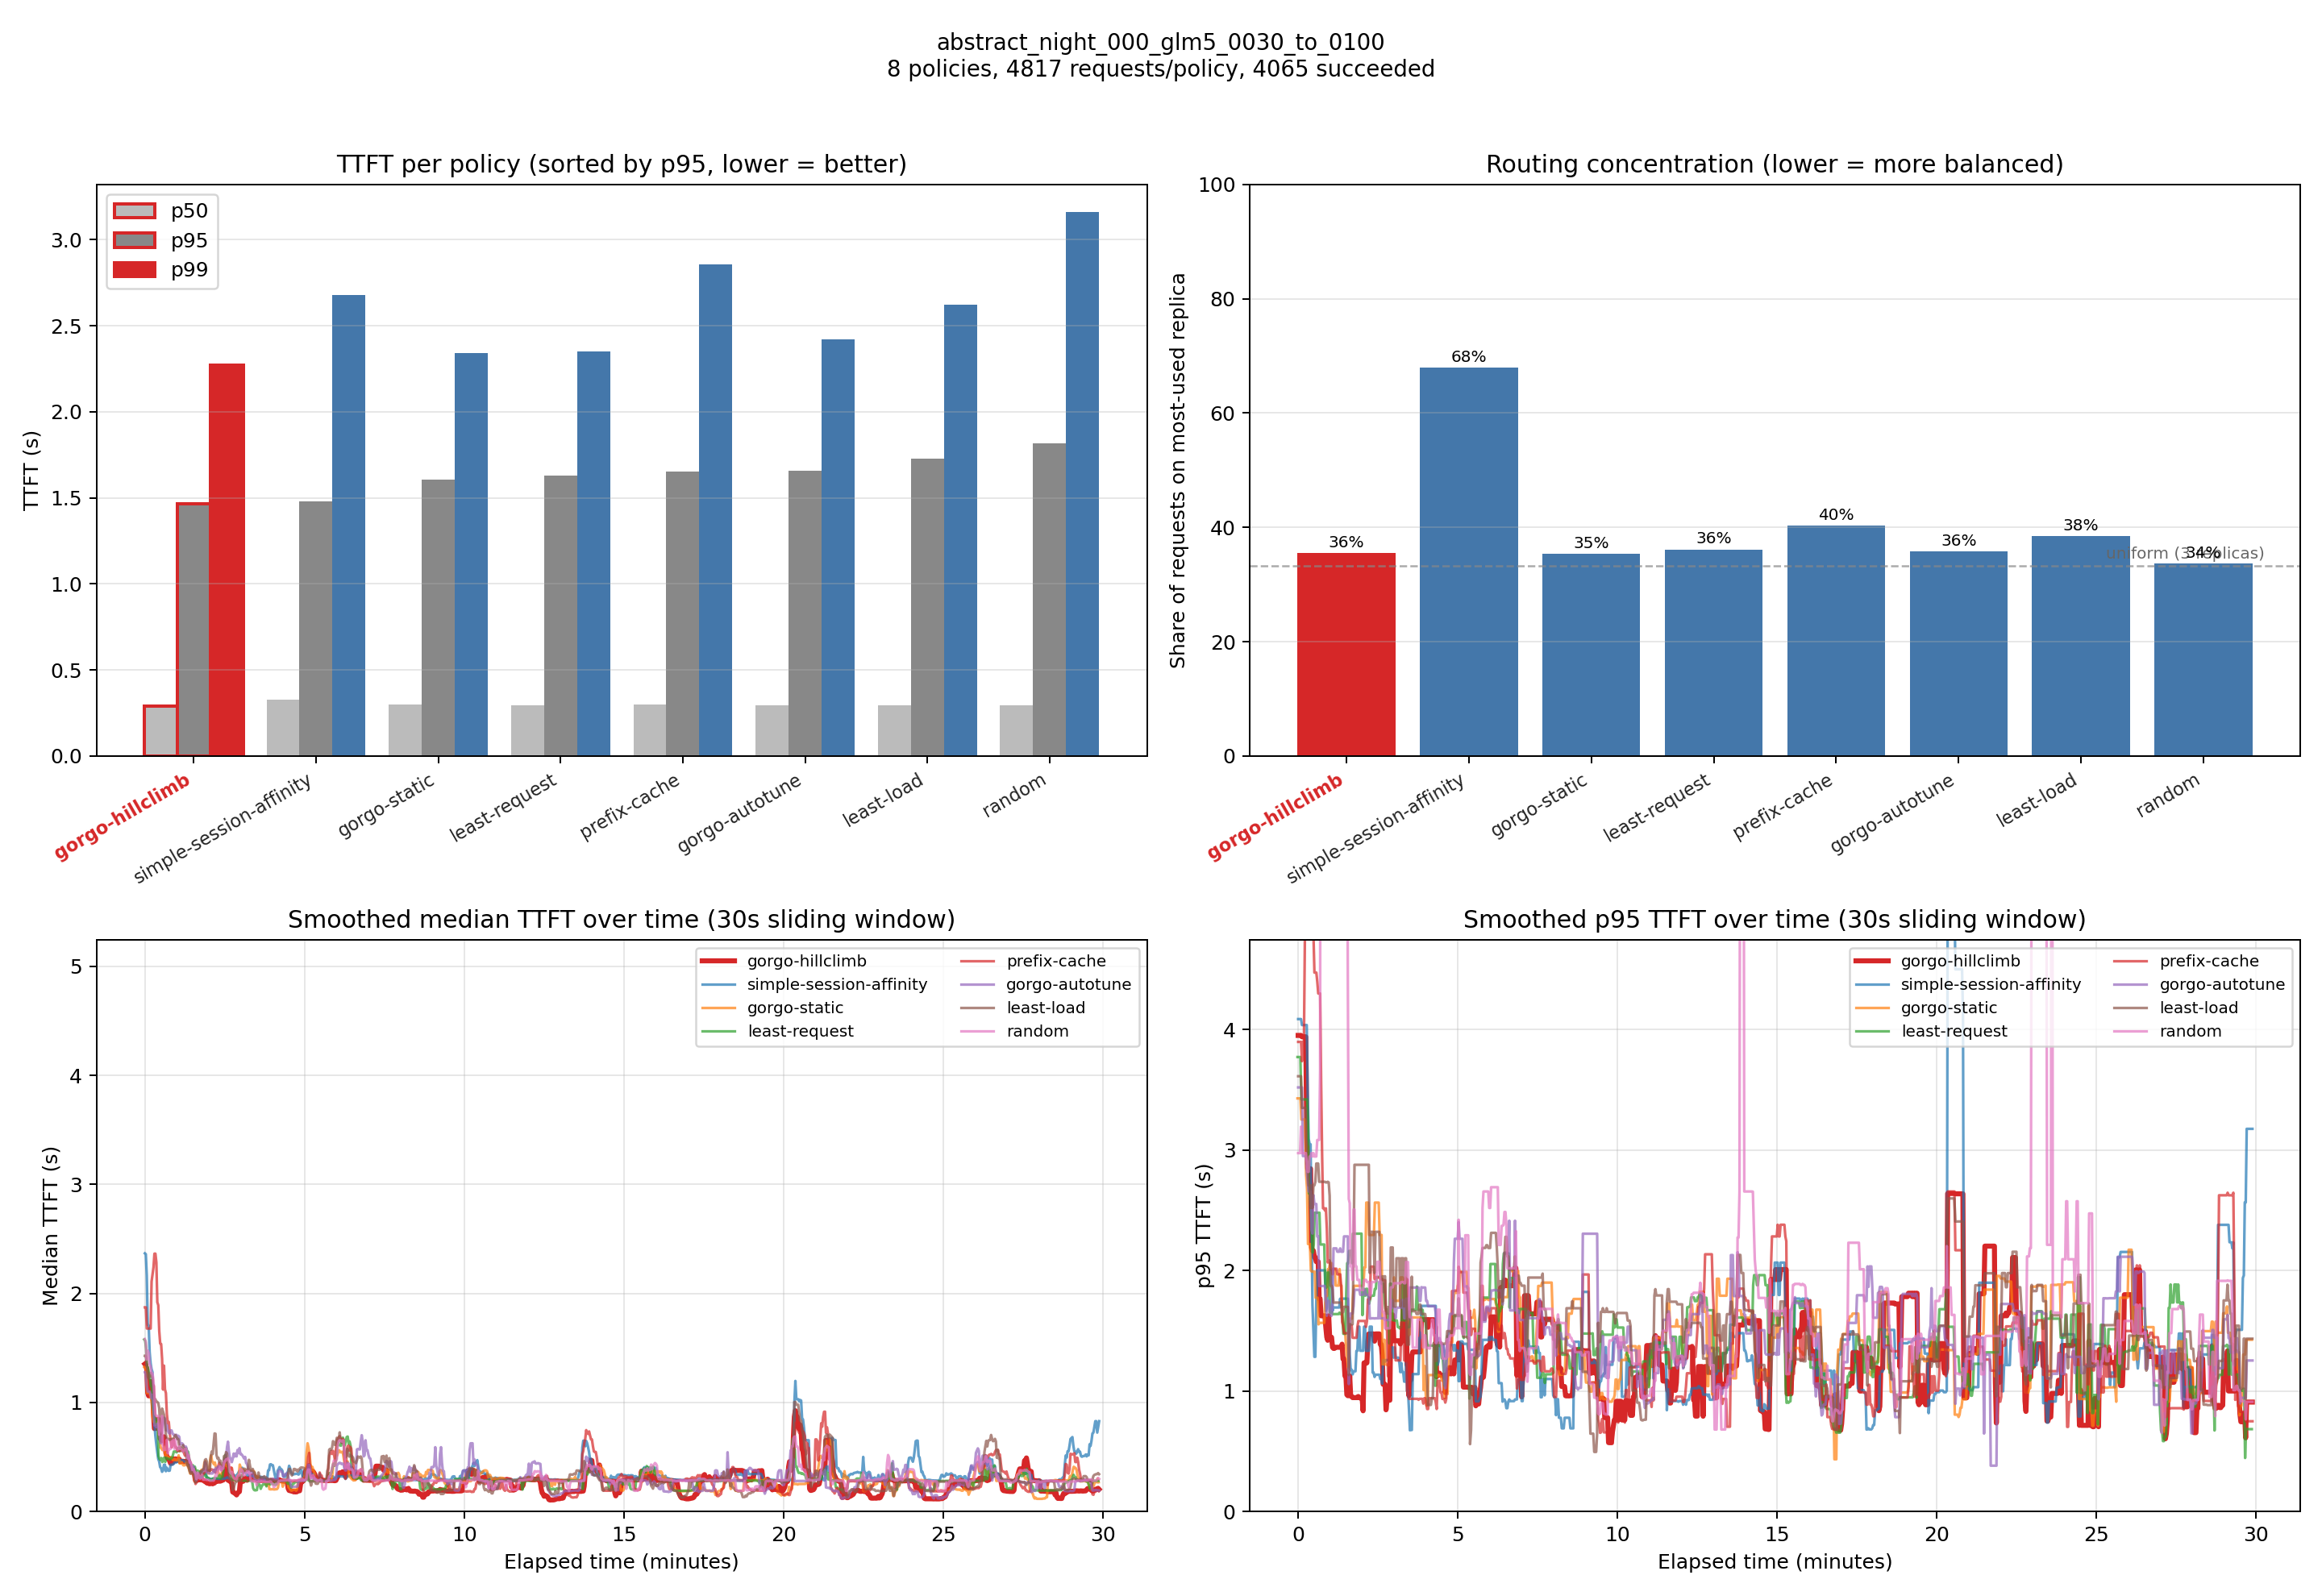
\includegraphics[width=\linewidth]{figures/glm5_w1_summary.png}
\caption{W1 (tuning window).}
\end{subfigure}\hfill
\begin{subfigure}{0.49\textwidth}
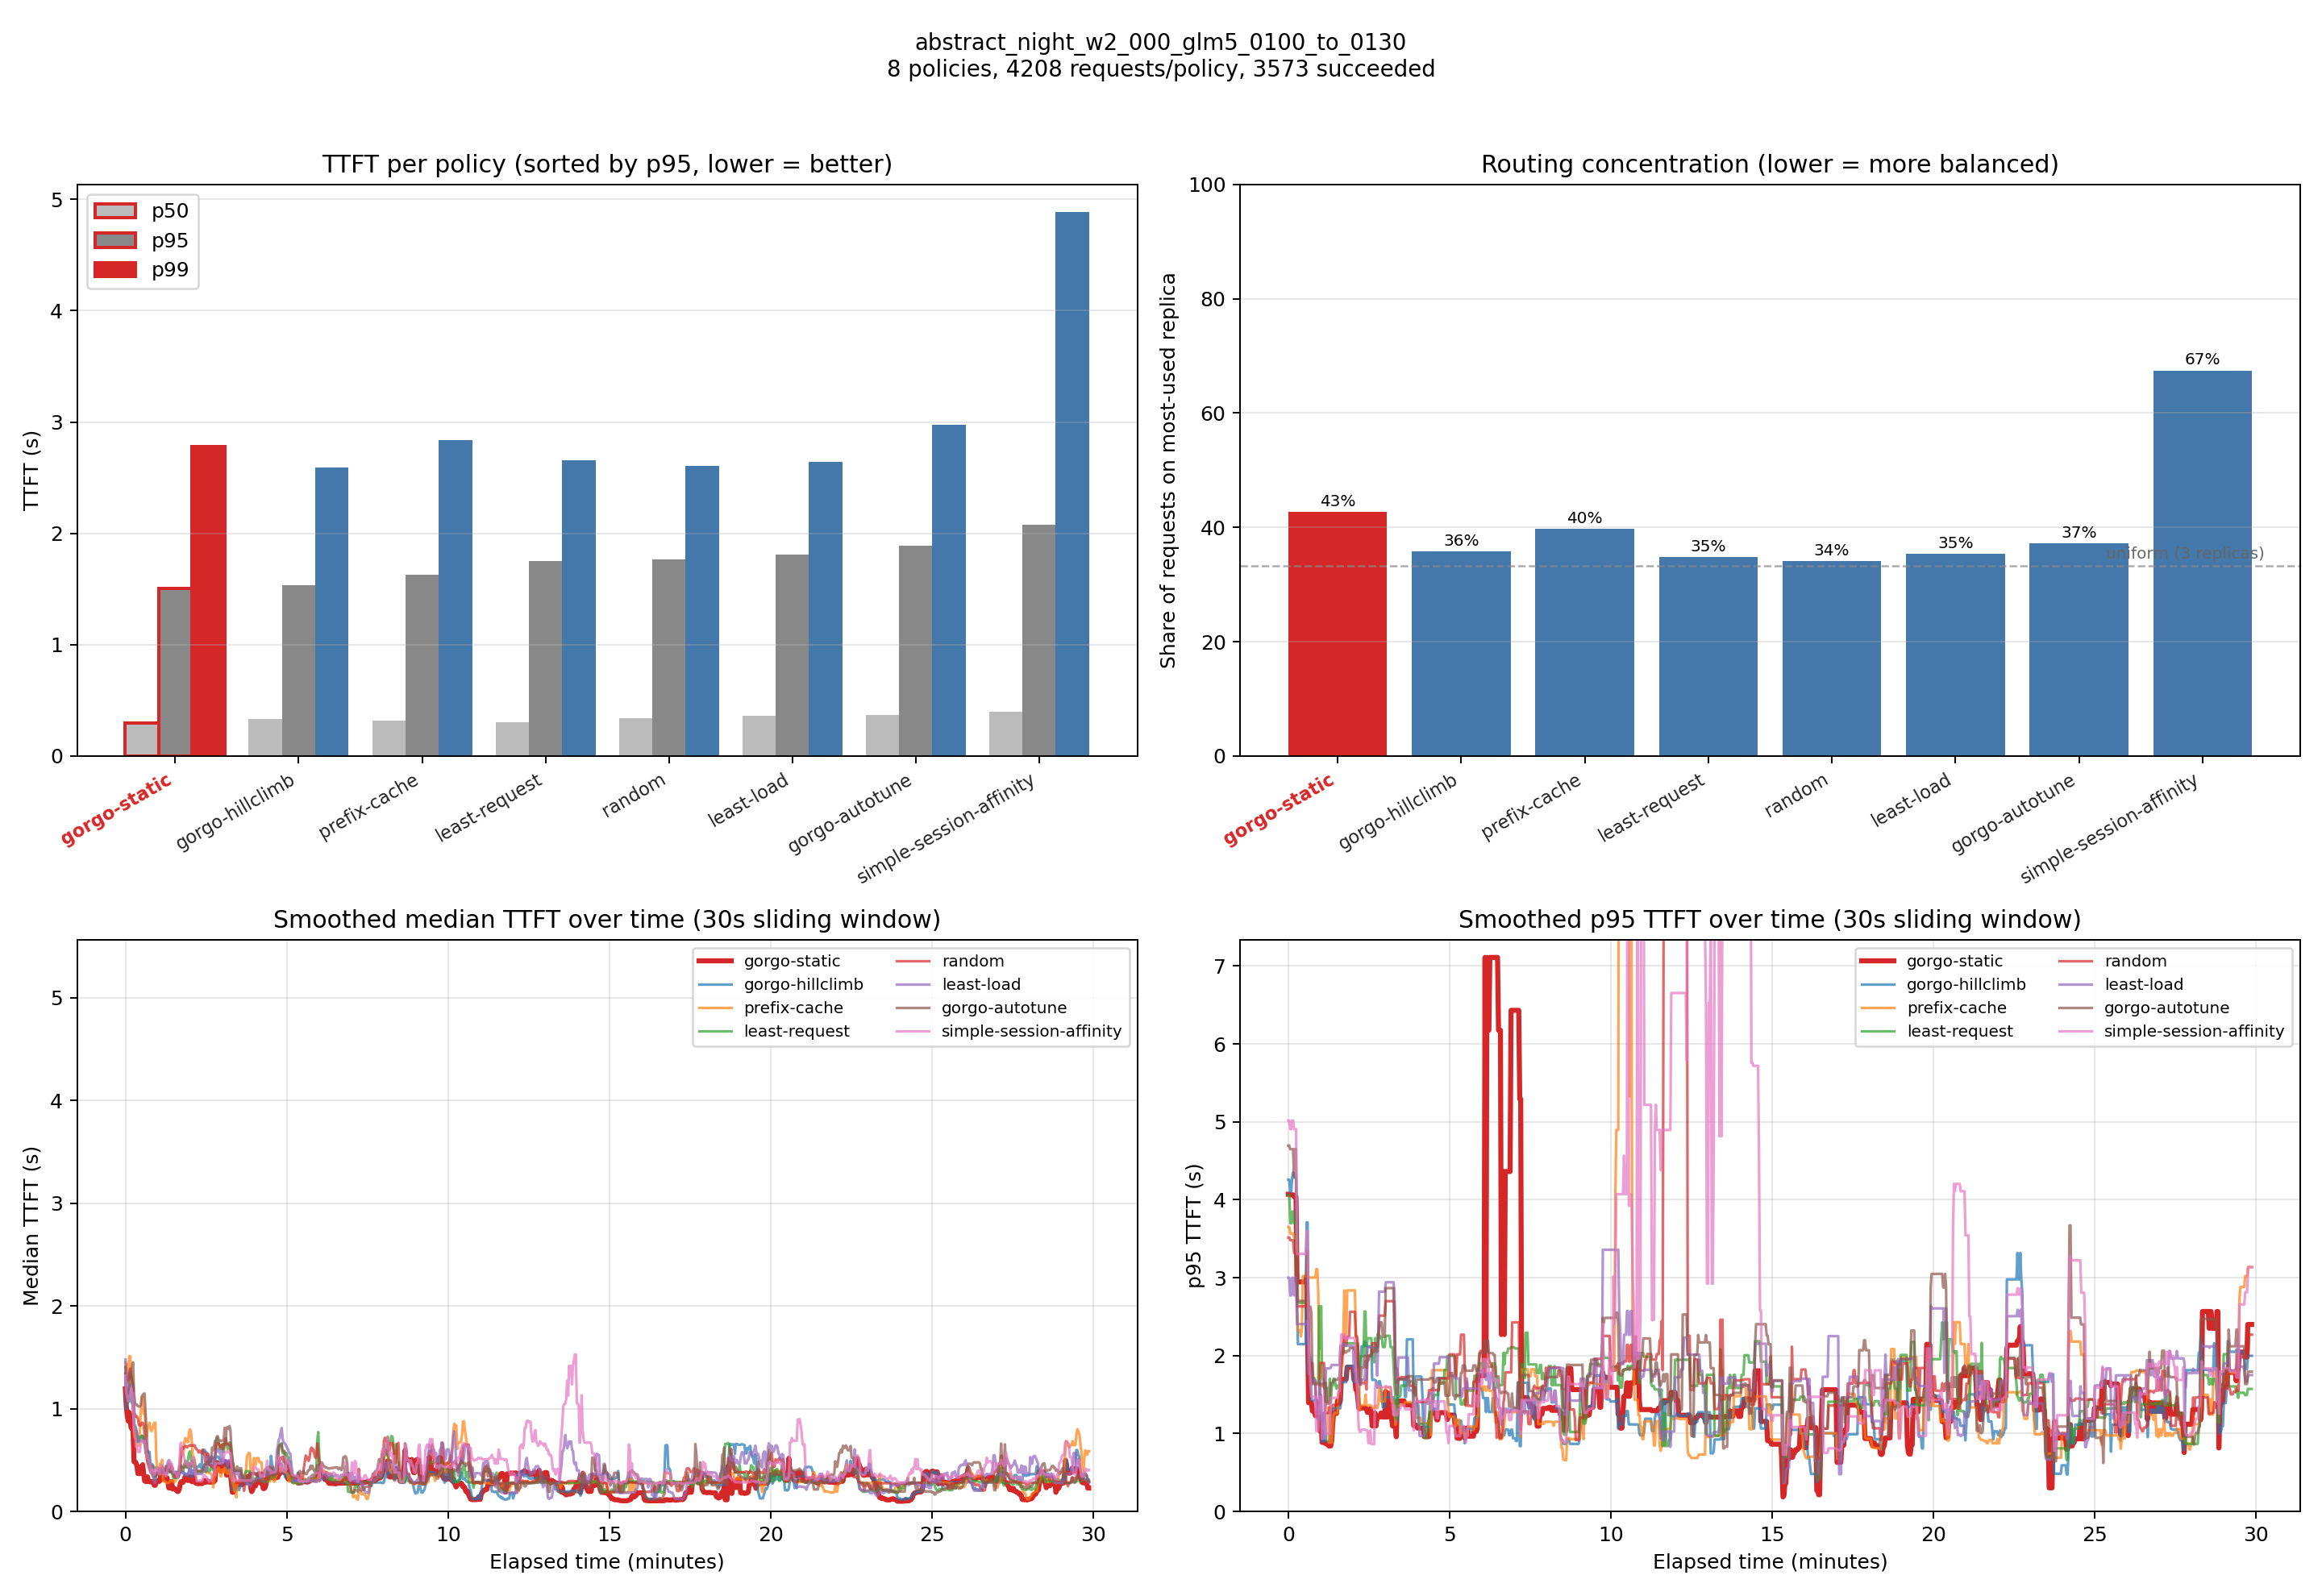
\includegraphics[width=\linewidth]{figures/glm5_w2_summary.png}
\caption{W2 (held-out evaluation window).}
\end{subfigure}
\caption{TTFT percentile sweep across all eight policies on the GLM-5.1 trace. The GORGO family achieves the lowest TTFT at every percentile in both windows, although the winning variant differs: \texttt{gorgo-hillclimb} sweeps p50/p95/p99 in W1, while in W2 \texttt{gorgo-static} (deploying W1-learned weights) takes p50 and p95 and \texttt{gorgo-hillclimb} takes p99.}
\label{fig:percentiles}
\end{figure}

\subsection{Tuning window}

In W1 (Table~\ref{tab:w1}), \texttt{gorgo-hillclimb} delivers the lowest p50 (0.288\,s), p95 (1.466\,s), and p99 (2.307\,s). The next-best p95 is \texttt{simple-session-affinity} at 1.482\,s, a 1.1\% gap. The \texttt{gorgo-static} configuration --- with manually-set weights of $0.07$ and $0.06$, never adjusted --- already beats every non-GORGO policy on p99 and ranks third on p95. \texttt{prefix-cache} is competitive on p95 (1.654\,s, mid-pack) but tail-degraded on p99 (3.017\,s) because it concentrates traffic onto warm-cache replicas and pays a queueing penalty. The p95 spread across all policies in W1 is 1.25$\times$ (1.466\,s for hillclimb, 1.828\,s for random). Starting from $t_{\mathrm{prefill}}=0.07$, $\alpha=0.06$, the (1+1)-ES converged to $t_{\mathrm{prefill}}\approx 0.983$ and $\alpha\approx 4.4\times 10^{-4}$ over the 30-minute window: $t_{\mathrm{prefill}}$ in the tuned model is a tiebreaking weight, not a physical rate, and the optimal load weight under a single-tenant trace is much smaller than a load-fairness heuristic would suggest, since SGLang's continuous batching already orders within a replica.

\subsection{Held-out evaluation window}

In W2 (Table~\ref{tab:w2}), \texttt{gorgo-static} --- deploying the W1-learned weights without further adjustment --- achieves the best p50 (0.294\,s) and p95 (1.510\,s). \texttt{gorgo-hillclimb} achieves the best p99 (2.595\,s). \texttt{gorgo-autotune}, the median-of-rates variant, performs worse than the static deployment in W2 (see below). The p95 spread between best and worst is 1.38$\times$, larger than W1's 1.25$\times$. The two GORGO variants together sweep all three percentiles in W2, but no single GORGO variant does. This is the ``GORGO sweeps every percentile in both windows'' claim, with ``GORGO'' denoting the family that shares Equation~\ref{eq:score}.

\textbf{Static beats hillclimb on p50/p95 in W2} because the W1-learned weights are near-optimal for the W2 distribution; continuing to tune on a similar distribution adds variance from each ES proposal (some accepted at marginally worse scores after the tolerance gate). This is a known property of (1+1)-ES under stationary objectives. A practical takeaway is that operators can run \texttt{gorgo-hillclimb} during a tuning window and freeze the result into \texttt{gorgo-static} for production. \textbf{The W2 p99 margin} between \texttt{gorgo-hillclimb} (2.595\,s) and \texttt{random} (2.612\,s) is 0.7\% --- inside the trace-level noise floor (\S\ref{sec:limitations}). The W1 sweep and W2 p50/p95 wins are 5--10\% margins, well outside that floor.

\textbf{Why \texttt{gorgo-autotune} underperforms.} The median-of-rates fit inverts Equation~\ref{eq:ttft} on the trailing 64 samples, but the rate $({\rm TTFT}-{\rm rtt})/{\rm uncached}$ is unstable when uncached counts are small (high cache hit), which inflates the rate and makes the policy over-weight prefill. The same per-replica median can be set by very different mixtures of fast cache hits and slow misses; the estimator treats them identically. \texttt{gorgo-hillclimb} avoids this because its objective integrates over the same mixture rather than trying to disentangle it. A cross-window comparison underscores the stability picture: \texttt{simple-session-affinity}'s p95 inflates 40.4\% W1$\to$W2 and its p99 by 75.4\% --- a hash-to-replica mapping cannot rebalance when a hash bucket spikes. \texttt{gorgo-static} is the only policy whose W2 p95 improves over W1 (--6.0\%).

\section{Discussion and Limitations}
\label{sec:limitations}

\textbf{Single-trace generalization.} The percentile-sweep claim rests on two consecutive 30-minute windows of one production trace, sharing model, fleet, hour-of-day, and arrival-rate band. W2 demonstrates that tuned weights survive a held-out window of the same workload, not arbitrary transfer across hours, days, or models.

\textbf{p99 noise floor.} Each window has $\sim$4{,}200--4{,}800 successful responses. p99 over a sample of this size has a standard error of approximately $\sigma_{\mathrm{TTFT}} / \sqrt{n \cdot 0.01 \cdot 0.99} \approx 0.05\,$s, putting the W2 p99 spread between \texttt{gorgo-hillclimb} and \texttt{random} (0.017\,s) inside one standard error. The W2 p50/p95 wins are several standard errors clear of zero.

\textbf{Single-tenant traffic.} Each policy ran on its own three-replica fleet, so cache state is single-tenant. Multi-tenant sharing changes the queue and cache dynamics that GORGO's load weight is meant to capture; convergence under non-stationary multi-tenant load is not validated here.

\textbf{Autotune failure.} The median-of-rates fit underperforms in W2: cost-model weights are best treated as black-box knobs (hillclimb) rather than identifiable physical rates. \textbf{No PD-disaggregation.} The fleet does not split prefill and decode \citep{distserve2024,splitwise2024}; the score would need an additional term. \textbf{No engine-internal signals.} GORGO uses only metrics that an HTTP-fronted SGLang/vLLM server exposes, not scheduler-internal information \citep{kvflow2025,lpc2025} that would tighten the prefill estimate.

\section{Related Work}
\label{sec:related}

\textbf{Prefix caches and reuse.} RadixAttention \citep{sglang2024} stores per-request KV state in a radix tree on the engine; PagedAttention \citep{vllm2023} enables prefix sharing through paged memory. KVLink \citep{kvlink2025}, ChunkKV \citep{chunkkv2025}, KVFlow \citep{kvflow2025}, and Learned Prefix Caching \citep{lpc2025} make the cache more efficient on each replica but do not decide which replica serves a request.

\textbf{Routing and scheduling.} Mooncake \citep{mooncake2025} is a KV-cache-centric architecture and the source of our trace format. AIBrix \citep{aibrix2024} provides the baseline policies (least-request, least-load, prefix-cache, power-of-two). k-LPM \citep{klpm2025} formulates LLM scheduling under TTFT constraints as NP-hard and proposes an algorithm interpolating between FCFS and longest-prefix-match. DLPM/D$^2$LPM \citep{dlpm2025} target fairness with locality. Llumnix \citep{llumnix2024} migrates requests across replicas. Multi-LLM training-free routers \citep{routerwu2025} address model selection, not cache-aware routing within one model. Splitwise \citep{splitwise2024} and DistServe \citep{distserve2024} disaggregate prefill from decode; SpecEdge \citep{specedge2025} is edge-assisted. GORGO commits to a single scalar score per replica with online weight tuning, requires no engine modifications, and deploys on a stock OpenAI-compatible fleet. The (1+1)-ES tuner follows Rechenberg \citep{rechenberg1973}; Bayesian or bandit-based alternatives are plausible but not benchmarked here.

\section{Conclusion}
\label{sec:conclusion}

We characterize a workload regime --- long-context, multi-turn, high prefix-reuse production traffic --- where standard LLM-serving routing heuristics each leave performance on the table because they pick one signal out of three (cache locality, replica load, network cost). On a 411{,}000-request production trace where 53.7\% of input tokens are part of a previously-seen prefix from the same user, three variants of a joint cost model collectively achieve the lowest TTFT at every percentile (p50, p95, p99) on both a tuning and a held-out evaluation window, against seven baseline policies, on a multi-region L40S:2 fleet with cross-region RTTs from 26 to 466\,ms. Per-percentile wins are not held by any single fixed weight setting; the best evaluation-window configuration is the one that froze the weights learned in the tuning window. The cost model and tuner fit on a stock HTTP gateway and require no offline profiling.

\bibliographystyle{plainnat}
\bibliography{references}

\newpage

\section*{NeurIPS Paper Checklist}

\begin{enumerate}

\item {\bf Claims}\\
Question: Do the main claims made in the abstract and introduction accurately reflect the paper's contributions and scope?\\
Answer: \answerYes{}\\
Justification: The abstract claims (i) public datasets underrepresent long-context multi-turn traffic, (ii) we evaluate routing policies on a production trace with quantified differences, and (iii) GORGO sweeps every TTFT percentile in both a tuning and an evaluation window. Section~\ref{sec:characterization} quantifies (i), Section~\ref{sec:results} reports (iii). We are explicit in the introduction and in Section~\ref{sec:limitations} that ``GORGO'' refers to a family of variants and that the W2 p99 margin is at the noise floor.

\item {\bf Limitations}\\
Question: Does the paper discuss the limitations of the work performed by the authors?\\
Answer: \answerYes{}\\
Justification: Section~\ref{sec:limitations} lists single-trace generalization, the W2 p99 noise floor, the single-tenant assumption, the failure of \texttt{gorgo-autotune} to recover physical rates, and the absence of PD-disaggregation in the fleet.

\item {\bf Theory assumptions and proofs}\\
Question: For each theoretical result, does the paper provide the full set of assumptions and a complete (and correct) proof?\\
Answer: \answerNA{}\\
Justification: The paper presents a closed-form additive cost model and an online optimizer; it does not state theorems with formal proofs.

\item {\bf Experimental result reproducibility}\\
Question: Does the paper fully disclose all the information needed to reproduce the main experimental results?\\
Answer: \answerYes{}\\
Justification: Section~\ref{sec:setup} specifies the model, regions, hardware, fleet topology, concurrency, trace windows, and per-window seeding for the GORGO variants. Section~\ref{sec:method} gives Equation~\ref{eq:score}, the (1+1)-ES configuration, and the median-of-rates fit. The reproducibility statement at the end of this checklist enumerates the four canonical paths in the released artifact.

\item {\bf Open access to data and code}\\
Question: Does the paper provide open access to the data and code, with sufficient instructions to faithfully reproduce the main experimental results?\\
Answer: \answerYes{}\\
Justification: The proxy, policies, trace builder, experiment controller, and the public-dataset characterization scripts are released. The GLM-5.1 production trace is not redistributable; we release the public-dataset characterization (LMSYS, WildChat) and the experiment controller in full so that the evaluation methodology is reproducible end-to-end on either public set.

\item {\bf Experimental setting/details}\\
Question: Does the paper specify all the training and test details?\\
Answer: \answerYes{}\\
Justification: Section~\ref{sec:setup} specifies model, hardware, regions, concurrency, trace windows, max input tokens, and per-window seeding for adaptive policies. The (1+1)-ES configuration ($\sigma_0=0.5$, $\sigma_{\min}=0.05$, $\sigma$ decay $0.817$, success window 8, target rate $0.2$, hop 16, window 64) is given in Section~\ref{sec:method}.

\item {\bf Experiment statistical significance}\\
Question: Does the paper report error bars suitably and correctly defined or other appropriate information about the statistical significance of the experiments?\\
Answer: \answerYes{}\\
Justification: We compute an approximate p99 standard error in Section~\ref{sec:limitations} and show that the W2 p99 spread between \texttt{gorgo-hillclimb} and \texttt{random} is inside one standard error. The W1 sweep and W2 p50/p95 wins are several standard errors clear of zero.

\item {\bf Experiments compute resources}\\
Question: For each experiment, does the paper provide sufficient information on the computer resources?\\
Answer: \answerYes{}\\
Justification: Each policy runs on a dedicated 3-replica fleet of L40S:2 SGLang servers serving Qwen3.5-35B-A3B-FP8, plus one CPU proxy. Eight policies $\times$ two windows = 16 fleet-runs, each $\sim$30 minutes wall clock plus warmup, on three regions. Total GPU-hours: $\sim$24 (16 runs $\times$ 0.5\,h $\times$ 3 replicas).

\item {\bf Code of ethics}\\
Question: Does the research conducted in the paper conform with the NeurIPS Code of Ethics?\\
Answer: \answerYes{}\\
Justification: The work concerns LLM-serving routing infrastructure, uses anonymized/aggregated prefix-trie statistics on public datasets, and uses a production trace under terms of service that permit research replay. No individuals are identifiable from the released aggregates.

\item {\bf Broader impacts}\\
Question: Does the paper discuss both potential positive societal impacts and negative societal impacts?\\
Answer: \answerYes{}\\
Justification: Routing improvements reduce the energy and dollar cost of serving large LLMs at fixed quality. Negative impacts: lower-cost serving may accelerate deployment of LLMs in settings where deployment is socially harmful (mass surveillance, mass content generation). The contributions of this paper are infrastructure-level and do not affect model capability.

\item {\bf Safeguards}\\
Question: Does the paper describe safeguards for responsible release of data or models with high risk for misuse?\\
Answer: \answerNA{}\\
Justification: We do not release datasets or models. The released code is a routing proxy and a load-balancing policy library; it has no inherent dual-use beyond LLM-serving infrastructure.

\item {\bf Licenses}\\
Question: Are creators or original owners of assets (e.g., code, data, models) properly credited and are the license and terms of use explicitly mentioned and properly respected?\\
Answer: \answerYes{}\\
Justification: SGLang, vLLM, and AIBrix are cited and used under their published licenses. LMSYS-Chat-1M and WildChat-4.8M are cited and used under their respective dataset licenses. The Qwen3 model is cited and used under its model card terms.

\item {\bf New assets}\\
Question: Are new assets introduced in the paper well documented and is the documentation provided alongside the assets?\\
Answer: \answerYes{}\\
Justification: The released proxy, policy library, experiment controller, and trace builder are documented in the repository's top-level documentation files. Spec and manifest files referenced by the controller are stored alongside the controller.

\item {\bf Crowdsourcing and research with human subjects}\\
Question: For crowdsourcing experiments and research with human subjects, does the paper include the full text of instructions given to participants and screenshots, if applicable, as well as details about compensation?\\
Answer: \answerNA{}\\
Justification: No human subjects.

\item {\bf Institutional review board (IRB) approvals or equivalent for research with human subjects}\\
Answer: \answerNA{}\\
Justification: No human subjects.

\item {\bf Declaration of LLM usage}\\
Question: Does the paper describe the usage of LLMs if it is an important, original, or non-standard component of the research methodology?\\
Answer: \answerNA{}\\
Justification: LLM serving infrastructure is the object of study. No LLM is used as a research methodology component (no LLM-judge, LLM-rewriter, etc.). Authors used LLMs for routine writing assistance only.

\end{enumerate}

\newpage

\section*{Reproducibility statement}

The experiments in this paper are driven by a single Modal application that launches a fleet, configures policies, and replays a Mooncake-format trace per policy. The four canonical paths in the released artifact are:

\begin{itemize}
\item \path{specs/policy_matrix_abstract_night.json} --- W1 spec (eight policies, manual GORGO starter weights);
\item \path{specs/policy_matrix_abstract_night_w2.json} --- W2 spec (eight policies, GORGO seeded with W1-learned weights);
\item \path{experiment_runner/policy_matrix_app.py} --- experiment controller;
\item \path{data_processing/build_mooncake_trace.py} --- trace builder.
\end{itemize}

The W1 and W2 manifests, per-window result CSVs, and summary plots in this paper are produced by running the controller against these specs and post-processing the per-policy stats with the released analysis scripts. The GLM-5.1 production trace is not redistributable; the public-dataset characterization (LMSYS, WildChat) reproduces with no proprietary inputs and uses the same trie-based prefix accounting described in Section~\ref{sec:characterization}.

\end{document}
